\documentclass[a4paper,11pt]{article}
\pdfoutput=1 % if your are submitting a pdflatex (i.e. if you have
             % images in pdf, png or jpg format)

\usepackage{jinstpub} % for details on the use of the package, please
                     % see the JINST-author-manual


\title{\boldmath On-field performance evaluation for the Silicon Photomultipliers of the Muon Telescope}
% Online temperature correction of SiPM bias voltage depending for the Muon Telescope

%% %simple case: 2 authors, same institution
%% \author{A. Uthor}
%% \author{and A. Nother Author}
%% \affiliation{Institution,\\Address, Country}

% more complex case: 4 authors, 3 institutions, 2 footnotes
\author[a,2]{J. S\'anchez-Villafrades,}
\author[b,1]{J. Pe\~na-Rodr\'iguez,\note{Corresponding author.}}
\author[b,2]{J. Pisco-Guabave}
\author[b,c,2]{L. A. N\'u\~nez}
\author[d,e,2]{and H. Asorey}

% The "\note" macro will give a warning: "Ignoring empty anchor..."
% you can safely ignore it.

\affiliation[a]{Escuela de Ingenier\'ia El\'ectrica, Electr\'onica y de Telecomunicaciones, Universidad Industrial de Santander,\\ Bucaramanga-Colombia}
\affiliation[b]{Escuela de F\'isica, Universidad Industrial de Santander,\\ Bucaramanga-Colombia}
\affiliation[c]{Departamento de F\'isica, Universidad de Los Andes, M\'erida-Venezuela.} 
\affiliation[d]{Departamento F\'isica M\'edica, Centro At\'omico Bariloche, Comisi\'on Nacional de Energ\'{\i}a At\'omica,\\ Bariloche-Argentina}
\affiliation[e]{Instituto de Tecnolog\'{\i}as en Detecci\'on y Astropart\'{\i}culas (ITEDA),\\ Buenos Aires-Argentina.}

% e-mail addresses: only for the for corresponding author
\emailAdd{jesus.pena@correo.uis.edu.co}


\abstract{The Muon Telescope is an experiment for imaging volcanoes in Colombia using muography. Due to the on-field operation conditions of MuTe, a full characterization of the silicon photomultipliers (SiPM) implemented in the particle tracking system depending on temperature variations is mandatory. In this work, we characterize the breakdown voltage, gain and noise at the MuTe SiPMs (Hamamatsu S13360-1350CS) for typical temperatures of the observation place spanning from 0$^{\circ}$C to 40$^{\circ}$C. We demonstrated that the discrimination threshold for the MuTe hodoscope must be above 5 p.e. to avoid contamination due to the SiPM noise caused by dark count, cross-talk and after-pulse. Furthermore, we assess the MuTe counting rate for an 8 p.e. threshold during day-night temperature variations.}

% a closed-loop control for the SiPMs bias is recommended to compensate the SiPM breakdown voltage (i.e. the event rate) variability due to the environment temperature.}


\keywords{Muography, Silicon Photomultipliers, Breakdown Voltage, Instrumental Noise}

\arxivnumber{xxxx.xxxxx} % only if you have one

% \collaboration{\includegraphics[height=17mm]{example-image}\\[6pt]
%   XXX collaboration}
% or

%\collaboration[c]{on behalf of XXX collaboration}

% if you write for a special issue this may be useful
%\proceeding{N$^{\text{th}}$ Workshop on X\\
%  when\\
%  where}

\begin{document}
\maketitle
\flushbottom

\section{Introduction}
\label{sec:intro}

%SiPMs play an important role in particle detection experiments applied in several fields from high energy physics to geology. 

Muography is a non-invasive technique for imaging anthropic and geologic structures by measuring the crossing muon flux using sensitive hodoscopes. In the last years, several applications have been developed such as detection of hidden materials in containers \cite{Blanpied2015}, archaeological building scanning \cite{Morishima2017, GomezEtal2016}, nuclear plant inspection \cite{Fujii2013}, nuclear waste monitoring, underground cavities \cite{Saracino2017}, the overburden of railway tunnels \cite{ThompsonEtal2019} and vulcanology \cite{Tanaka2005, Tanaka2009, Lesparre2010, Lesparre2011, Lesparre2012, TanakaOlah2019}.

Hodoscopes are mainly built by nuclear emulsions \cite{Morishima2017, NAGAMINE2016}, gaseous chambers \cite{Sehgal2016, Fehr2012, Bouteille2016, Olh2018} and scintillators \cite{Fujii2013, Lesparre2012, Tanaka2009, Nagamine1995, Aguiar2015, Tang2016}. Last ones are widely used due to their easy implementation, low cost and robustness against environmental variables as humidity, temperature and atmospheric pressure \cite{Procureur2018}. The measurement principle of scintillation counters can be explained in twofold: an ionizing particle interacts with the crystal lattice, exciting electrons in the valence band and transferring them to bound states called excitons. Then excitons are de-excited by recombination emitting photons in the near-ultraviolet spectrum. Taking into account the absorption length of the ultraviolet light is quite short, some dopants are added to the basic material in order to obtain a light output in a longer wavelength. The resultant emission wavelength range of scintillator is not fully adjusted to the sensitivity of photosensors (Photomultipliers or SiPMs), therefore it is necessary to add a wavelength shifting fiber. Consequently, the emission spectrum matches the spectral sensitivity of the sensor enhancing the photodetection efficiency \cite{Grupen2008}.

SiPMs offer an ideal solution for high granularity hodoscopes to be deployed in volcanic areas because of their small dimensions, robustness, and low power consumption \cite{Ambrosino2014}. SiPMs are composed of a dense array of small photon avalanche diodes (PAD) operating in Geiger mode. When a photon interacts with a SiPM microcell, an avalanche process starts generating a photocurrent flowing through a quenching resistor which causes that the diode bias drops below the breakdown value preventing further Geiger-mode avalanches. The electrical pulses generated by the SiPM are directly related to the number of incident photons. The main drawback of SiPMs is that performance parameters like gain, photodetection efficiency (PDE) and breakdown voltage are very sensitive to temperature variations.

The Muon Telescope (MuTe) is an hybrid detector composed by an hodoscope and a Water Cherenkov Detector (WCD) which will be installed in one of the most dangerous volcanoes in Colombia, the Cerro Machin, located at 2750 m.a.s.l. on the Cordillera Central near to the municipality of Cajamarca \cite{AsoreyEtal2017B}. The MuTe hodoscope consists of two scintillation panels each of 30 $\times$ 30 strips 120 cm length and 4 cm width. Each strip has an 1.8 mm hole for a multi-cladding wavelength shifting (WLS) fiber (Saint-Gobain BCF-92)  with $1.2$ mm diameter, an absorption peak at $410$ nm and an emission peak of $492$ nm \cite{SaintGobain2018}. The WLS fiber is coupled, with a silicon photomultiplier (SiPM, Hamamatsu S13360-1350CS) \cite{Hamamatsu2018}. The SiPM has a photosensitive area of $1.3 \times 1.3 \textrm{ mm}^2$, $667$ pixels, a fill factor of $74\%$, a gain from $10^5$ to $10^6$ and a photon-detection efficiency of $40 \%$ at $450 \textrm{nm}$ \cite{pena2019calibration, PenaRodriguezEtal2018}.

Due to the MuTe operates on-field under variable environmental conditions, characterization of SiPM parameters and its temperature dependence plays a key step in the detector calibration process. Here we evaluate the MuTe SiPMs taking into account their breakdown voltage, gain, dark count, cross-talk and after-pulse in several temperature and over-voltage conditions. In section \ref{sec:exp} we describe the experimental setups and the data acquisition system for the SiPM evaluation. In section \ref{sec:res} we show the results of the breakdown voltage, gain and noise characterization. In section \ref{sec:obs} the temperature conditions at the Cerro Mach\'in volcano and their affectation on the MuTe mechanical structure are shown. In section \ref{sec:temp} flux and temperature measurements of the MuTe tracking system in on-field conditions are shown. As a summary, in section \ref{sec:conc} we close with the main conclusions and remarks of this work.


\section{Experimental setups and Data Acquisition System}
\label{sec:exp}

\subsection{Breakdown voltage setup}

The first experimental setup is used for measuring the SiPM dark current depending on temperature and bias voltage. A sketch of the setup is shown in Figure \ref{fig:set1}. The SiPM is placed on an isolated aluminum holder whose temperature is controlled by two Peltier cells (TEC1-12706 from Hebei I.T) is sensed by means of an LM35. A proportional-integral-derivative (PID) control implemented in a microcontroller Atmega328 generates two pulse-width-modulate (PWM) signals whose duty cycle depends on the calculated error between the sensed temperature and the pre-established set-point. The signals are optically coupled to a full-bridge driver for controlling the direction (cooling or heating) and amplitude (fast or slow) of the current flowing through the Peltier cells.

\begin{figure}[htbp]
\centering % \begin{center}/\end{center} takes some additional vertical space
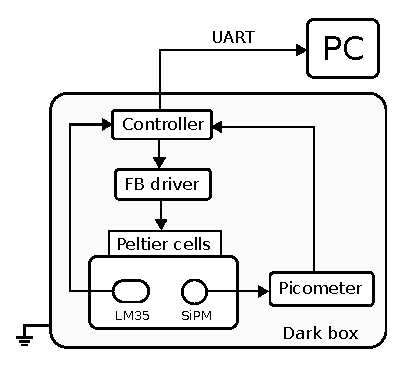
\includegraphics[width=.5\textwidth]{Figures/ExpSet1.eps}
\caption{\label{fig:set1} Experimental setup for measuring the SiPM dark current in darkness conditions. The SiPM is positioned in the aluminum holder inside the dark box. The holder temperature is controlled via Peltier cells by means a PID controller implemented in the Atmega328.}
\end{figure}

The SiPM S13360-1350CS is biased with a C11204 power module covering a voltage range from 40 to 60 V. The SiPM dark current is measured by a 2 nA accuracy picometer. Moreover, the SiPM bias voltage and temperature are recorded individually by a 10 bit analog to digital converter with a sampling rate of 1 Hz. All the setup components are placed inside a grounded dark box in order to avoid external light contamination and electromagnetic interference.


\subsection{Gain and noise setup}

In order to estimate the gain and noise variability of the SiPM depending on the temperature and overvoltage, we need to extract its photoelectron and charge spectrum. To achieve this aim, the SiPM must be stimulated with a pulsed light source with a wavelength matching the SiPM spectral sensitivity range and a pulse width of the order of a few ns \cite{Georgiev2016, Eigen2019}.

In this case, the SiPM temperature was controlled in the same way that in the breakdown voltage setup. The signals generated by the SiPM were amplified by 94 using a low noise current feedback operational amplifier (OPA691 from Texas Instruments) and digitized by a Red Pitaya ADC channel at a sampling frequency of 125 MSPS and 14 bits resolution.

The LED pulser generates an ultra-short (< 10 ns) 480 nm light pulse with a frequency of 500 Hz. A 50 cm WLS fiber (Saint-Gobain BCF-92) transports the blue light towards the SiPM, at the same time, a square signal triggers the DAQ system. Both, the trigger and the SiPM signals are sent via 50-ohm coaxial cables (RG-58). A vector of 500 samples (4 uS) with a time step of 8 ns contains the information of the pulse shape. A sketch of the setup is shown in Figure \ref{fig:set2}..

% In Figure \ref{fig:signal} we see a set of 150 pulses, where B is the signal portion before stimulation and A after stimulation. 

\begin{figure}[htbp]
\centering % \begin{center}/\end{center} takes some additional vertical space
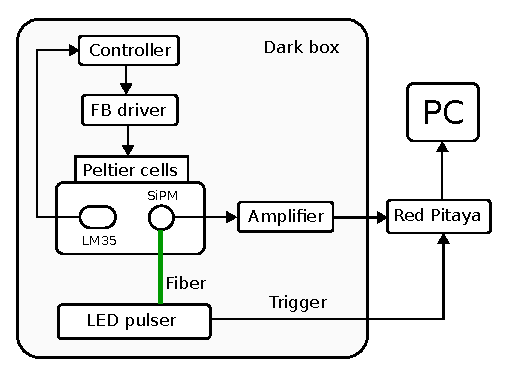
\includegraphics[width=.6\textwidth]{Figures/ExpSet2.eps}
\caption{\label{fig:set2} Experimental setup for measuring the gain and noise of the SiPM S13360-1350CS under stimulated conditions. The SiPM is stimulated by a 480 nm pulsed light of $\sim$ 10 ns width at 500 Hz. The SiPM signal is digitized by the Red Pitaya at 14 bits/125 MSPS.}
\end{figure}

% \begin{figure}[htbp]
% \centering % \begin{center}/\end{center} takes some additional vertical space
% 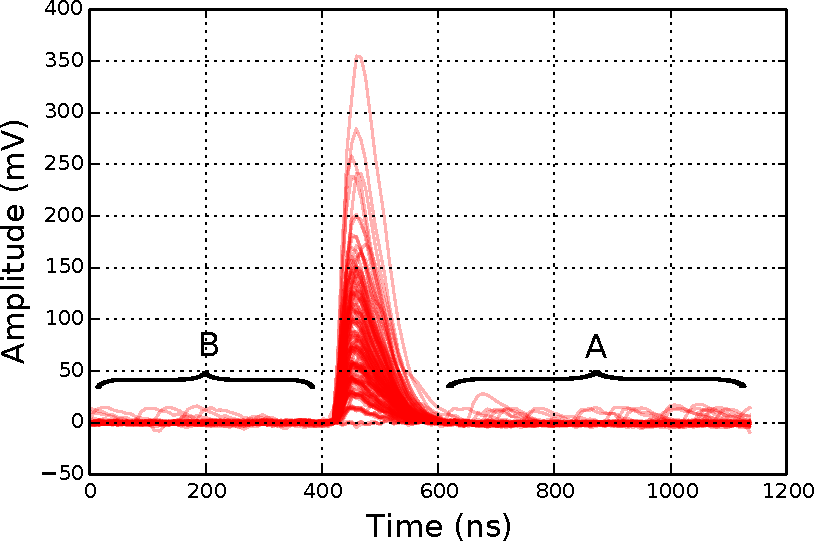
\includegraphics[width=.6\textwidth]{Figures/100P_1350CS.pdf}
% \caption{\label{fig:signal} Example of 150 pulses recorded by the DAQ system. Each pulse is split in three parts, before stimulation (B), during stimulation, and after stimulation (A), in order to carry out the noise analysis.}
% \end{figure}


\section{SiPM calibration}
\label{sec:res}

\subsection{Breakdown voltage}
The breakdown voltage (V$_{br}$) is the point where the SiPM enters in Geiger mode. Such a point can be established using several methods \cite{Nagy2017}. In this case, we use the tangent method which consists of finding the interception between a tangent line fitted to the IV (dark current vs bias voltage) curve and the baseline. In Figure \ref{fig:Vbr} we show the SiPM IV curve at 25$^{\circ}$C where the V$_{br}$ was found to be about 52.3 V.

\begin{figure}[htbp]
\centering % \begin{center}/\end{center} takes some additional vertical space
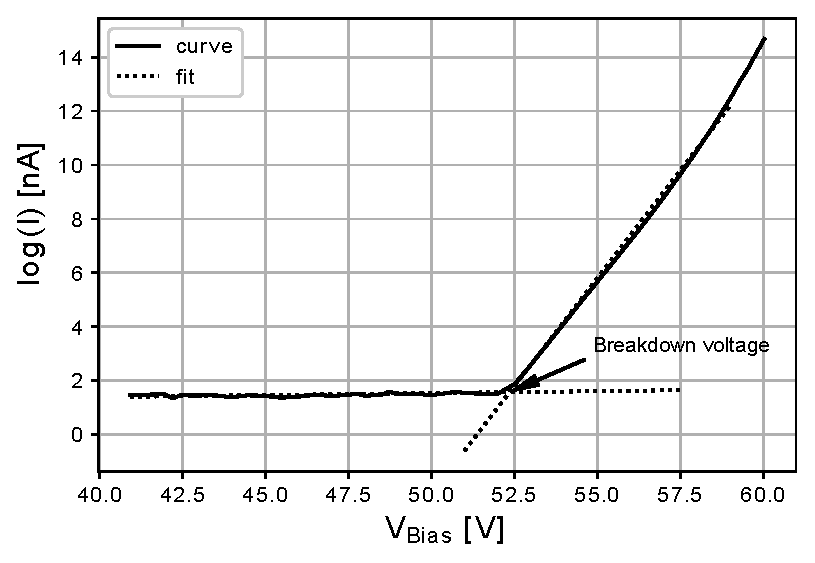
\includegraphics[width=.55\textwidth]{Figures/cal_voltaje_ruptura.eps}
\caption{Breakdown voltage value found using the tangent method for the IV curve of SiPM S13360-1350CS operating at 25$^{\circ}$C. The V$_{br}$ (52.3 V) is located at the intersection between the fit and the base line.}
\label{fig:Vbr} 
\end{figure}

We measured the IV curves from 40 to 60 V for temperatures between 0$^{\circ}$C and 40$^{\circ}$C with 5$^{\circ}$C steps as shown in Figure  \ref{fig:IVcurve} (left). In the Geiger region the IV slope increases with the temperature reaching a dark current above 400 nA at 40 $^{\circ}$C. Moreover, the breakdown voltage has a linear relation with temperature decreasing with a ratio of 41.7 mV/$^{\circ}$C as is shown in \ref{fig:IVcurve} (right). In on-field applications, an adaptive bias voltage to compensate for temperature changes in the SiPM must be taken into account to guarantee a stable gain and low noise levels \cite{Eigen2019}.

\begin{figure}[htbp]
\centering % \begin{center}/\end{center} takes some additional vertical space
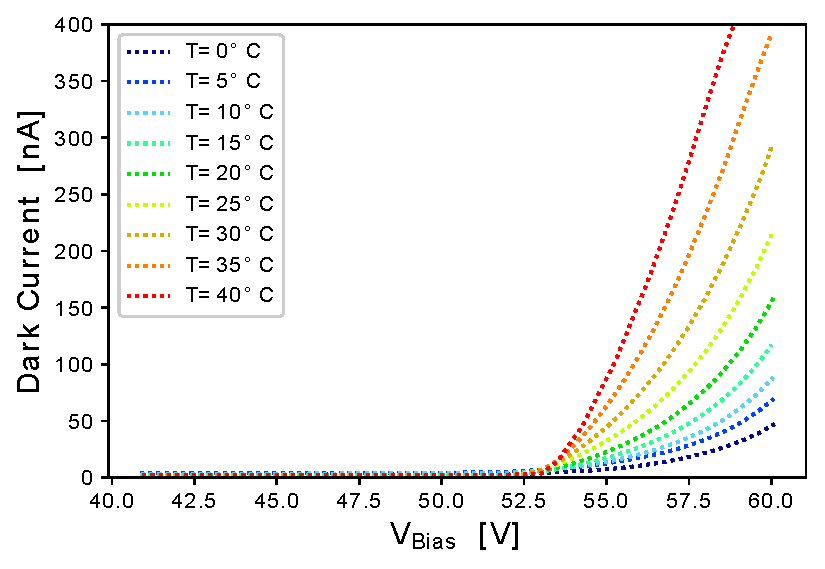
\includegraphics[width=.47\textwidth]{Figures/dc_13360.eps}
\qquad
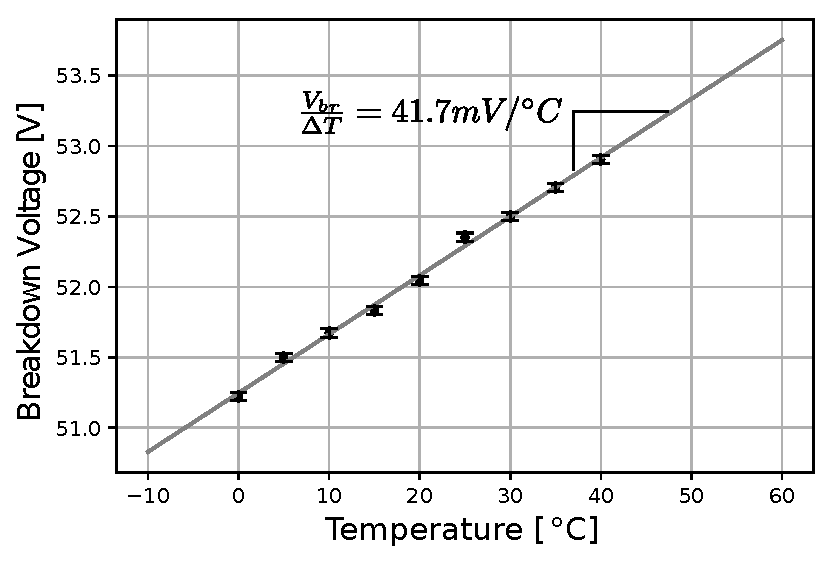
\includegraphics[width=.47\textwidth]{Figures/Vbd_vs_T_S13360.eps}
\caption{\label{fig:IVcurve} Temperature dependence of the breakdown voltage for the SiPM S13360-1350CS from Hamamatsu. (Left): IV curves ranging from 0$^{\circ}$C to 40$^{\circ}$C. (Right): $V_{br}$ variance ratio depending on the temperature.}
\end{figure}

\subsection{Charge spectrum and gain}

The gain of a SiPM microcell is defined as the ratio of the output charge to the charge on an electron $e$ \cite{Acerbi2019}. The output charge can be calculated as,

\begin{equation}
\label{eq:y:3}
Q = \frac{Q_{ADC}*V_{ADC}*\Delta_T}{RG_a}
\end{equation}
where $Q_{ADC}$ is the digitized area under pulse, $V_{ADC}$ is the equivalent voltage for one ADC unit, $\Delta_T$ is the digitization time step, $R$ is the input resistor and $G_a$ the gain of the electronics front-end. In Figure \ref{fig:charge} the charge spectrum of the SiPM operating at 56 V and 25$^{\circ}$C is shown.


\begin{figure}[htbp]
\centering % \begin{center}/\end{center} takes some additional vertical space
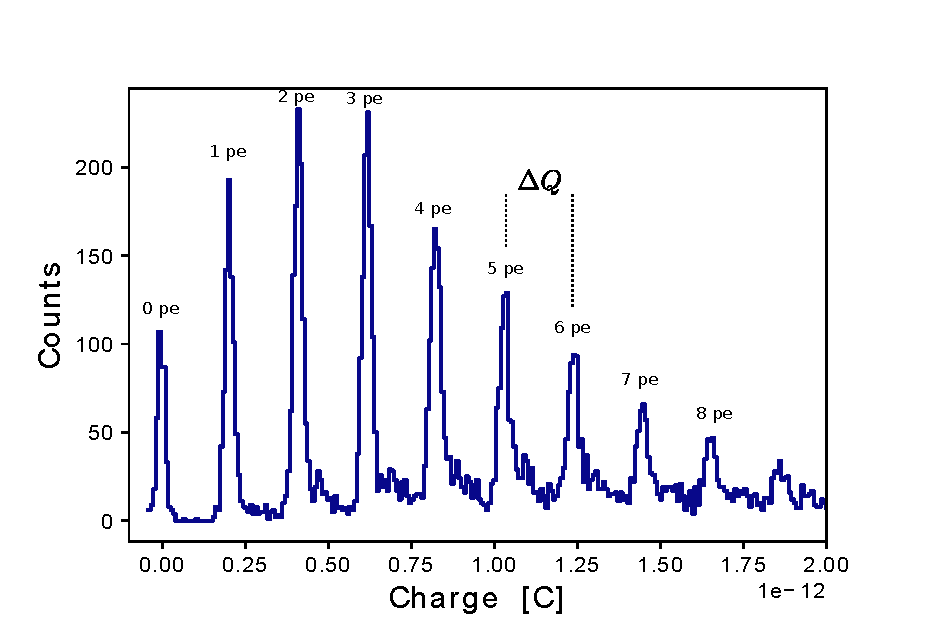
\includegraphics[width=.65\textwidth]{Figures/Charge.eps}
\caption{\label{fig:charge} Charge spectrum of the SiPM S13360-1350CS operating at 56V/25$^{\circ}$C. The first peak is the pedestal and the following represent the photoelectron equivalents. The $\Delta Q$ is the inter-peak charge which determines the SiPM gain.}
\end{figure}

The separation between two adjacent peaks $\Delta Q$ in the charge histogram corresponds to the charge from a single Geiger discharge. This can be used to accurately calculate the gain $G$ as follows,

\begin{equation}
\label{eq:y:3}
G = \frac{\Delta Q}{e}
\end{equation}

The SiPM gain depends on the bias voltage ($V_{bias} = V_{br} + \Delta$V), the higher the bias voltage the higher the gain. In order to estimate the gain dependence on the overvoltage ($\Delta V$) in the SiPM S13360-1350CS we measured three charge spectra for $\Delta$V = 1.7V, 2.7V, and 3.7V at 25$^{\circ}$C. In Figure \ref{fig:gain} the charge spectra for these cases are shown.

\begin{figure}[htbp]
\centering % \begin{center}/\end{center} takes some additional vertical space
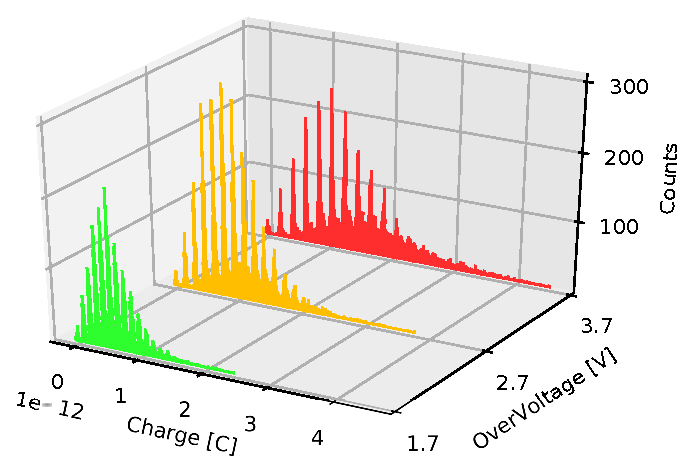
\includegraphics[width=.49\textwidth]{Figures/GainCharge.eps}
\quad
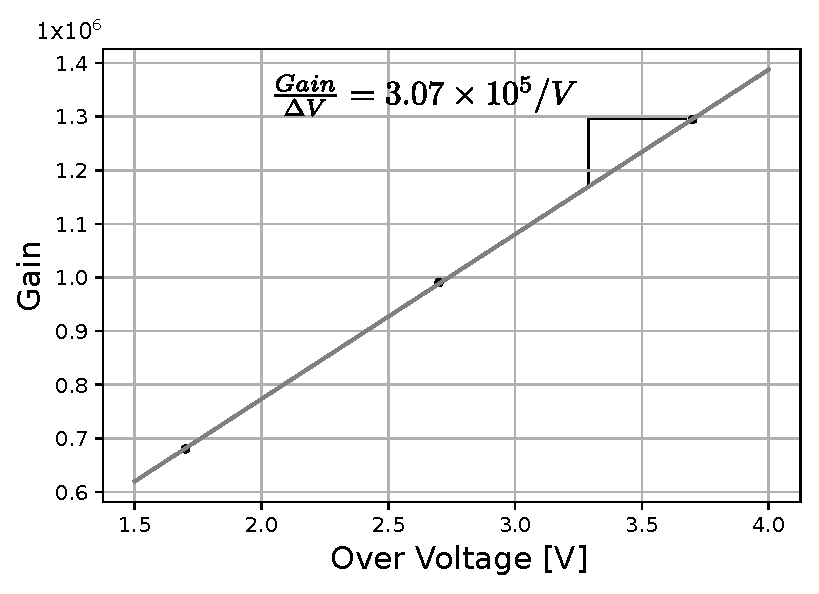
\includegraphics[width=.47\textwidth]{Figures/G_OV_1350CS.eps}
\caption{\label{fig:gain} (Left): Charge spectrum for $\Delta V=$1.7 V (green), 2.7 V (orange), and 3.7 V (red). (Right): Gain variation ratio depending on the overvoltage.}
\end{figure}

The separation between charge peaks grows as the overvoltage increases, indicating a gain increment. The gain change ratio depending on the overvoltage was estimated to be 3.07$\times10^5$/V, i.e., for $\Delta$V = 1.7V ($V_{bias} = 53$ V) the gain is roughly 0.7$\times10^6$ and $\Delta$V = 3.7V ($V_{bias} = 56$ V) the gain is 1.3$\times10^6$.

\subsection{Photoelectron spectrum}

SiPMs are composed of an array of APDs, all connected in parallel. The output pulse amplitude from SiPMs is proportional to the number of incident photons. The photoelectron (p.e.) spectrum determines the equivalent value (voltage or current) of a photon interacting with the active area of the SiPM. This value establishes the threshold for measuring dark count, crosstalk and afterpulse noise.

\begin{figure}[htbp]
\centering % \begin{center}/\end{center} takes some additional vertical space
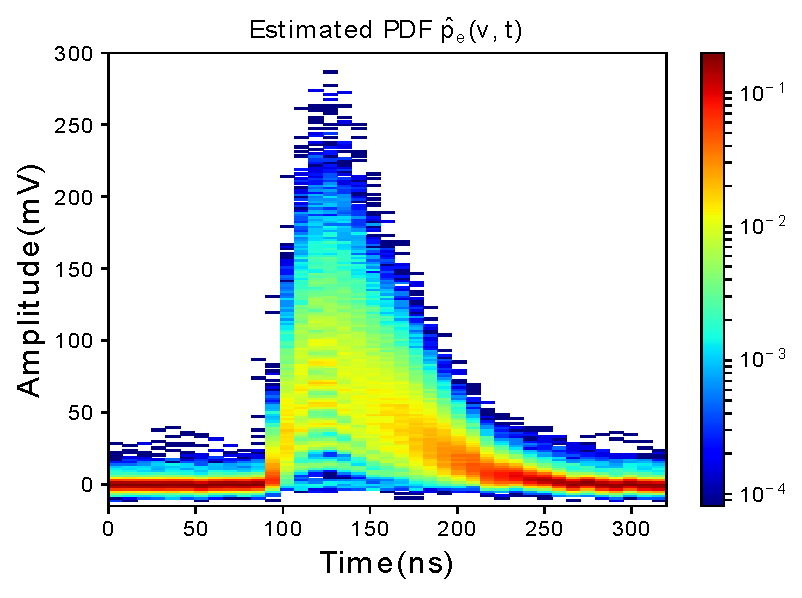
\includegraphics[width=.48\textwidth]{Figures/PDF_1350CS.eps}
%\qquad
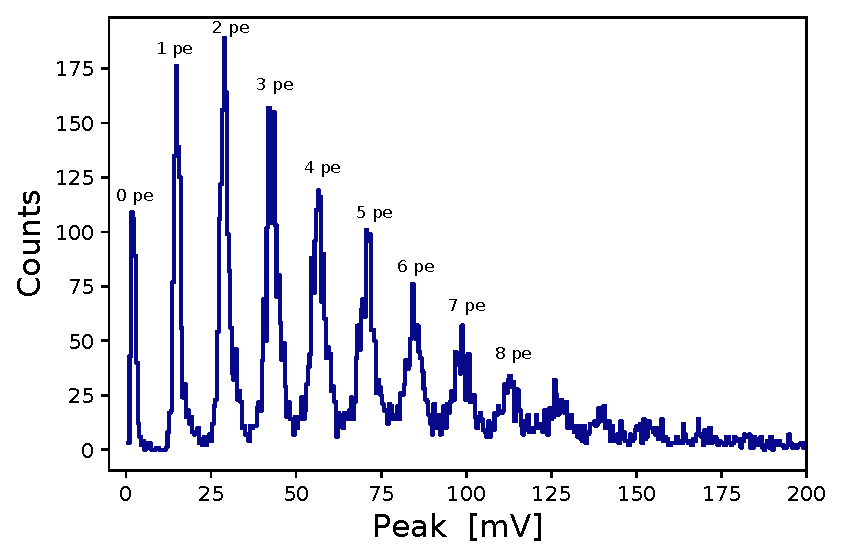
\includegraphics[width=.49\textwidth]{Figures/Peak_1350CS.eps}
\caption{\label{fig:peak} (Left): Waveform of the Hamamatsu S13360-1350CS under stimulation. Photo-electron spectrum resulting from integrating the area under pulse over a time window of 300 ns.}
\end{figure}

In Figure \ref{fig:peak} the persistence histogram (left) of the pulse shape and the peak histogram (right) for 10$^4$ pulses at 56 V/25$^{\circ}$C are shown.

A clear amplitude quantization is revealed with a high probability of occurrence at 1 and 2 p.e. where the pulses are mainly generated by the SiPM noise. The voltage value equivalent to 1 p.e is $\sim$13.5mV, therefore the threshold for measuring the SiPM dark count must be set at 13.5 mV and for the cross-talk at 27 mV.

\subsection{Noise}

SiPMs are affected by correlated noise (\textit{crosstalk} and \textit{afterpulses}) and non-correlated noise (dark count rate - DCR) \cite{Baudis2018}. These noise sources impose a lower limit of measurement in SiPM based experiments. We performed a noise analysis of the MuTe SiPMs taking into account its temperature and over-voltage dependency. Additionally, we established the minimum p.e. threshold above which the noise is negligible.

\subsubsection{Dark count rate}
The main source of noise in SiPMs is the DCR which appears as a consequence of avalanches processes fired by electrons thermally generated in the silicon crystal. The signals generated by thermal electrons and single-photons are identical. DCR is measured under dark conditions by counting events above a 0.5 p.e. threshold.

\begin{figure}[htbp]
\centering % \begin{center}/\end{center} takes some additional vertical space
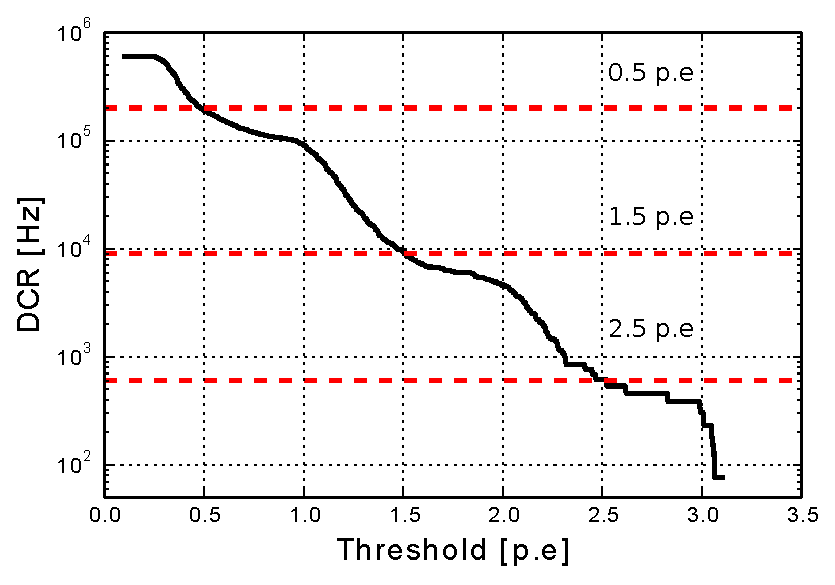
\includegraphics[width=.55\textwidth]{Figures/DCR_vs_th_pe_1350CS.eps}
\caption{\label{fig:DCR} Dark count rate as a function of signal threshold. The curve shape has three breaks at 0.5 p.e., 1.5 p.e. and 2.5 p.e.}
\end{figure}

The DCR is calculated as follows,
\begin{equation}
    DCR = \frac{N_{1pe}^B}{T^B N_p}
    \label{DCR_eq}
\end{equation}
where $N_{1pe}^B$ is the number of events above 0.5 p.e. in the time window ($T^B=1.6$ $\mu$s) before stimulation and $N_p$ is the total number of recorded events.

We measured the DCR for different thresholds spanning from 0.1 p.e. to 3.1 p.e at 56 V/25$^{\circ}$C as shown in Figure \ref{fig:DCR}. The resulting curve has a stepped shape because of the quantized nature of the SiPM pulses. At 0.5 p.e. the DCR is $\sim$ 2$\times 10^5$ Hz corresponding with the expected values provided by the SiPM S13360-1350CS datasheet which range between 0.9$\times 10^5$ Hz and 2.7$\times 10^5$ Hz.

The DCR drastically decreases while the measurement threshold increases. We found a DCR of 9$\times 10^3$ Hz at 1.5 p.e. and 6$\times 10^2$ Hz at 2.5 p.e. At 3.5 p.e. the DCR is expected to be negligible (< 10 Hz).

\begin{figure}[htbp]
\centering 
%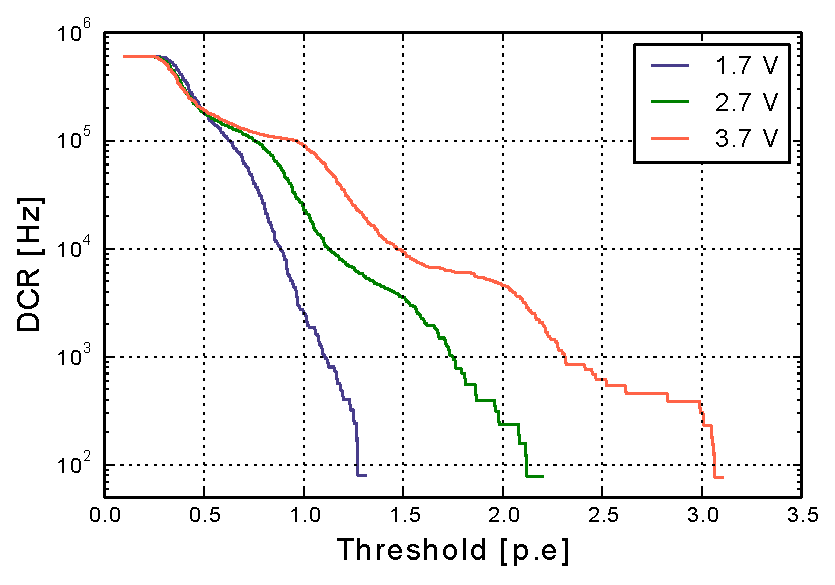
\includegraphics[width=.48\textwidth]{Figures/DCR_vs_th_1350CS.eps}
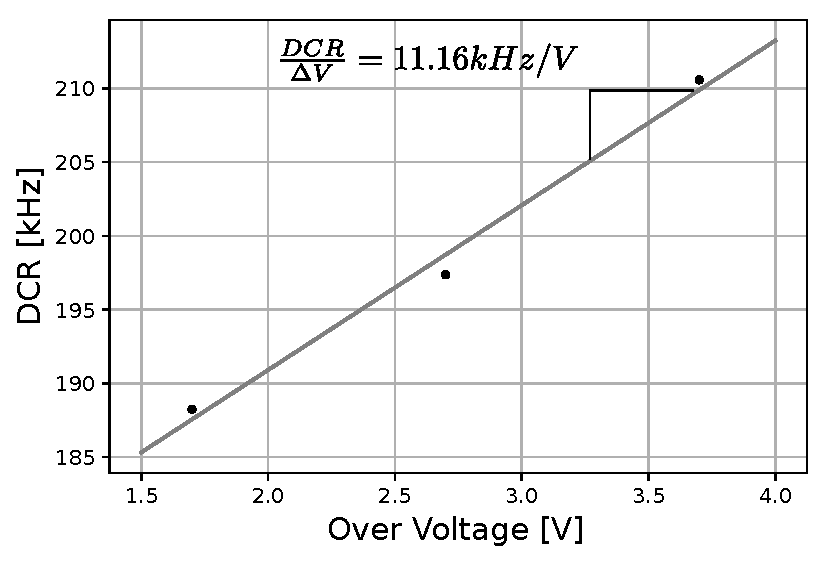
\includegraphics[width=.48\textwidth]{Figures/DCR_vs_ov_1350CS.eps}
\quad
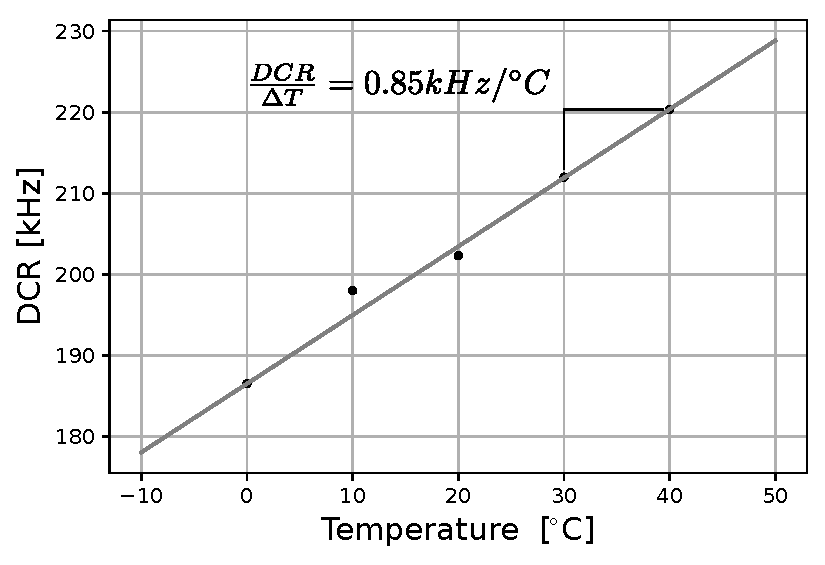
\includegraphics[width=.48\textwidth]{Figures/DCR_T_1350CS.eps}
\caption{\label{fig:DCRover} (Left): Dark count rate as a function of the overvoltage spanning from (1.7 V to 3.7 V) at 25$^{\circ}$C. (Right): Dark count rate as a function of temperature spanning from 0$^{\circ}$C to 40$^{\circ}$C at 56 V. The variation ratio is 0.85 kHz/$^{\circ}$C.}
\end{figure}

To characterize the DCR as a function of the overvoltage, we carried out DCR measurements for three cases (1.7 V, 2.7 V and 3.7 V) at 25$^{\circ}$C. The DCR increases as a function of the overvoltage with a ratio of $\sim$ 11.16 kHz/V as shown in Figure \ref{fig:DCRover} (Left). On the other hand, the temperature dependence of the DCR was evaluated from 0$^{\circ}$C to 40$^{\circ}$C at 56 V finding a ratio of 0.85 kHz/$^{\circ}$C as shown in Figure \ref{fig:DCRover} (Right).



\subsubsection{Afterpulsing and crosstalk}

Afterpulsing is generated by trapped electrons in silicon impurities during an avalanche process, these electrons are released few nanoseconds later creating new avalanches, that means, consecutive pulses \cite{Xu2017}. The amplitude of afterpulses increases with the retention time of the trapped electron. 

%In Figure \ref{fig:after} we show two examples of afterpulses following a primary pulse.

% \begin{figure}[htbp]
% \centering % \begin{center}/\end{center} takes some additional vertical space
% 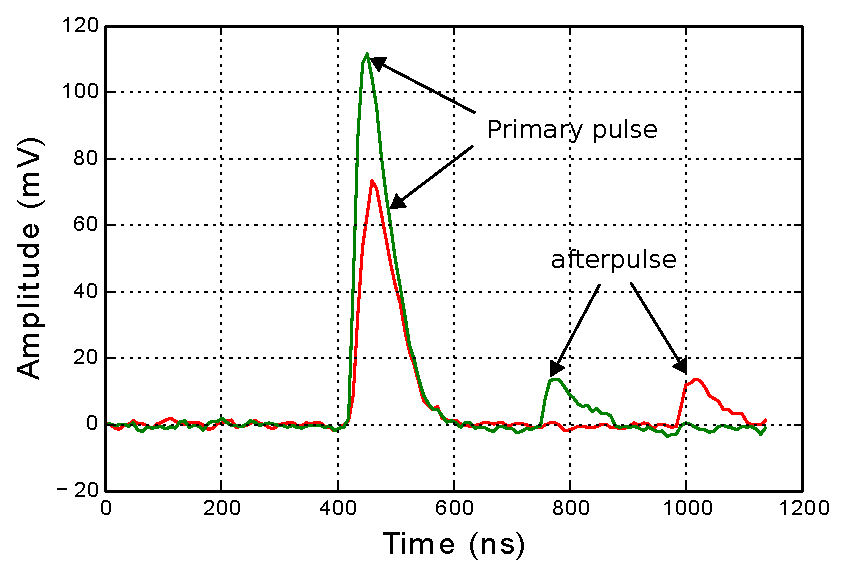
\includegraphics[width=.6\textwidth]{Figures/100P_1350CS_after.eps}
% \caption{\label{fig:after} Afterpulse examples for 5 p.e. (red) and 8 p.e. (green) primary events.}
% \end{figure}

The probability $P_{AP}$ of afterpulses is calculated as follows
\begin{eqnarray}
    P_{AP} &=& \frac{N_{1pe}^A-N_{1pe}^B}{N_p}\times 100
    \label{AP_eq}
\end{eqnarray}
where $N_{1pe}^A$ is the number of events above 0.5 p.e in the time window ($T^A = 1.6 \mu$ s) after the primary pulse. 

Crosstalk occurs when charge carriers inside the avalanche emit photons that interact with neighboring cells, generating secondary avalanches in such cells with amplitudes of 2 p.e. or 3 p.e.

%In Figure \ref{fig:cross} we show typical pulses generated by dark count (green), 2 p.e. crosstalk (blue) and 3 p.e. crosstalk (red).

% \begin{figure}[htbp]
% \centering % \begin{center}/\end{center} takes some additional vertical space
% 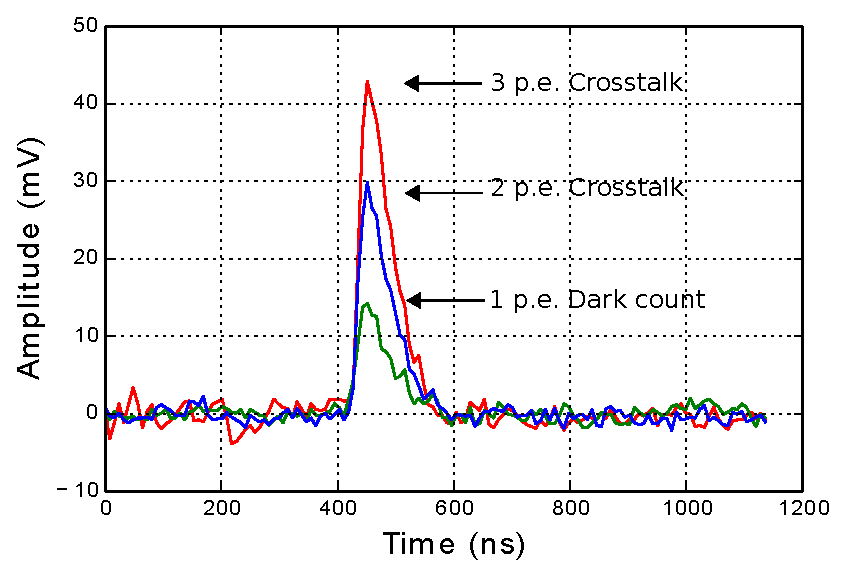
\includegraphics[width=.6\textwidth]{Figures/100P_1350CS_cross.eps}
% \caption{\label{fig:cross} Afterpulse of S13360-1350CS as a function of overvoltage ranging from 1 V to 4 V.}
% \end{figure}

The crosstalk probability is defined as
\begin{eqnarray}
    P_{CT} &=&\frac{N_{2p.e.}^B}{DCR}\times 100
    \label{CT_eq}
\end{eqnarray}
where $N_{2p.e.}^B$ is the number of events with an amplitude above 2 p.e before stimulation.

Figure \ref{fig:after_cross} (Right) shows the afterpulsing and crosstalk behavior depending on the SiPM overvoltage. Both parameters increase exponentially with the overvoltage, being the crosstalk always greater than afterpulsing. The afterpulse probability reaches 3$\%$ at 56 V/25$^{\circ}$C while the crosstalk probability rises up 5$\%$.

\begin{figure}[htbp]
\centering 
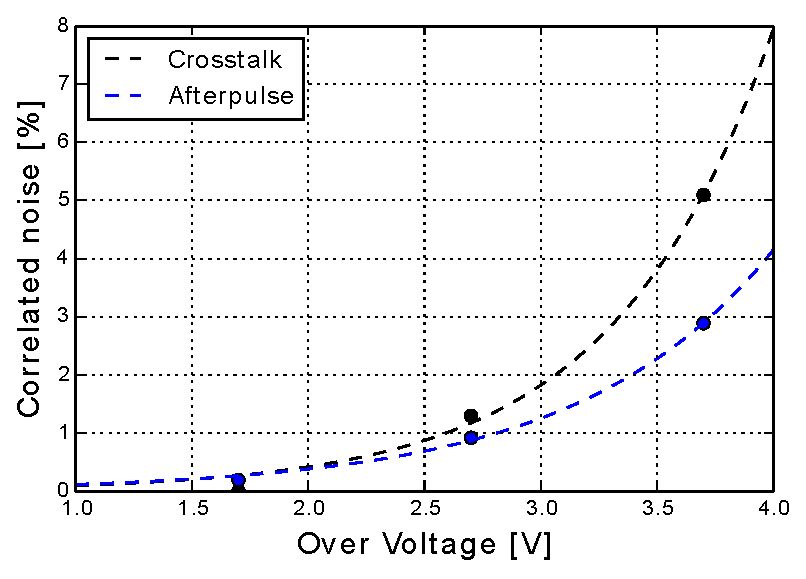
\includegraphics[width=.48\textwidth]{Figures/CorrNoise_vs_Ov_1350CS.eps}
\quad
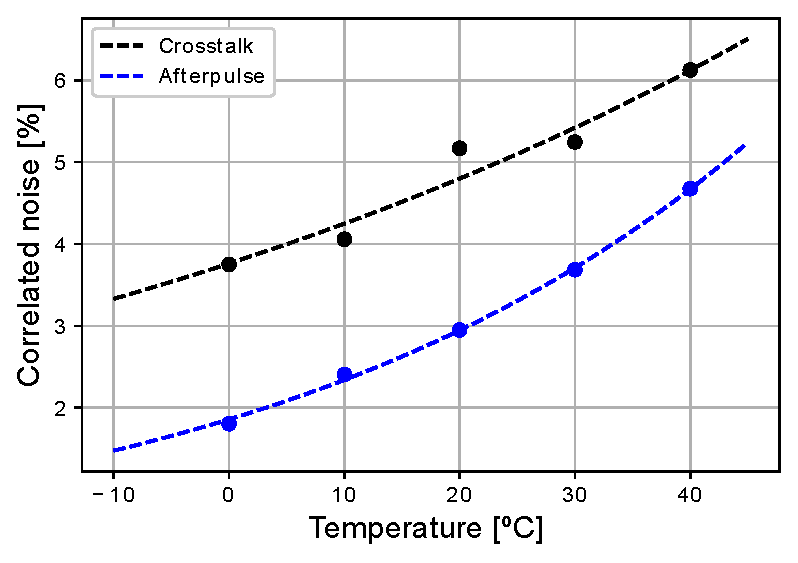
\includegraphics[width=.48\textwidth]{Figures/CorrNoise_vs_T_1350CS.eps}
\caption{MuTe-SiPM crosstalk (black line) and afterpulsing (blue line) depending on its overvoltage (left) and temperature (right).}
\label{fig:after_cross}
\end{figure}

The correlated noise dependency on temperature was analyzed by performing afterpulsing and crosstalk measurements from 0$^{\circ}$C to 40$^{\circ}$C at 56 V. The results are displayed on Figure \ref{fig:after_cross} (Left). At 0$^{\circ}$C the afterpulse probability is below 2$\%$ and the crosstalk below 4$\%$. The afterpulsing increases faster than crosstalk with the temperature, rising up almost 5$\%$ at 40$^{\circ}$C while crosstalk reaches 6$\%$ for the same temperature value.

In order to reduce the noise caused by dark count, crosstalk and afterpulse, we concluded that the ideal discrimination threshold for the scintillator hodoscope of MuTe must be above 5 p.e. On another hand, a closed-loop control of the SiPMs bias voltage is needed taking into account breakdown voltage shifting due to temperature variations and as result a modulation of the detection rate.

% \begin{figure}[htbp]
% \centering 
% 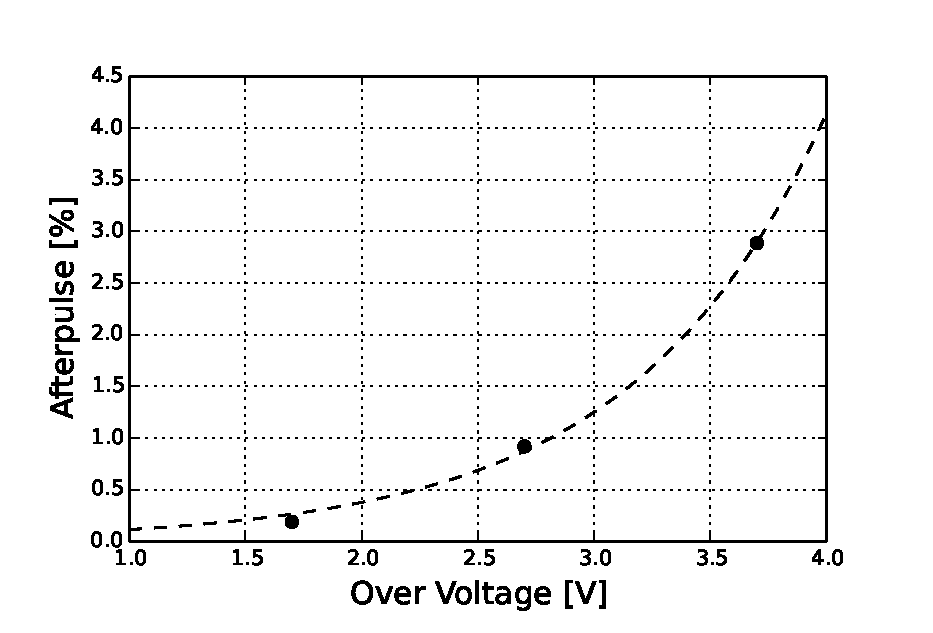
\includegraphics[width=.6\textwidth]{Figures/After_vs_Ov_1350CS.eps}
% \caption{\label{fig:after_Ov} Afterpulse as a function of overvoltage ranging from 1 V to 4 V.}
% \end{figure}

% \begin{figure}[htbp]
% \centering 
% \includegraphics[width=.6\textwidth]{Figures/Cross_vs_Ov_1350CS.eps}
% \caption{\label{fig:crossOv} Crosstalk of S13360-1350CS as a function of overvoltage ranging from 1 V to 4 V.}
% \end{figure}


\section{Operating temperature conditions of the MuTe}
\label{sec:obs}

\subsection{Weather at the Cerro-Machin Volcano}

The Cerro-Mach\'in volcano has typical weather conditions of the Andean mountains in Colombia with an average temperature of 16$^{\circ}$C, a relative humidity of 85 $\%$, and a maximum wind speed of 30 m/s according to the Colombian Hydrology, Meteorology and Environmental Studies Institute (IDEAM by its acronym in Spanish of \textit{Instituto de Hidrolog\'ia, Meteorolog\'ia y Estudios Ambientales}). During the rainy season, the temperature drops to 0$^{\circ}$C and during the dry season it rises up to 25$^{\circ}$C. The rainy season comes from April to May and October to November, and the dry season is usually from December to January and July to August. The day-night temperature variation at the Cerro-Mach\'in volcano is around 10$^{\circ}$C along the dry and rainy seasons.

\subsection{Heat transfer in the MuTe structure}

We performed a thermal analysis for computing the heat transfer by conduction, convection, and radiation along the MuTe mechanical structure taking into account the environmental temperature, solar radiation, cooling by wind, and heating by electronics power consumption. The simulation was carried out using the \textsc{Solidworks 3D CAD Modeling Software}. The simulation input parameters were the solar radiation (4.5 kWh m$^{-1}$day$^{-1}$), mean temperature (16$^{\circ}$C), maximum wind speed (30 m/s), the power dissipation (12.5 W), and the thermal features of the metallic chassis supporting the hodoscope and the WCD.


\begin{figure}[htbp]
\centering 
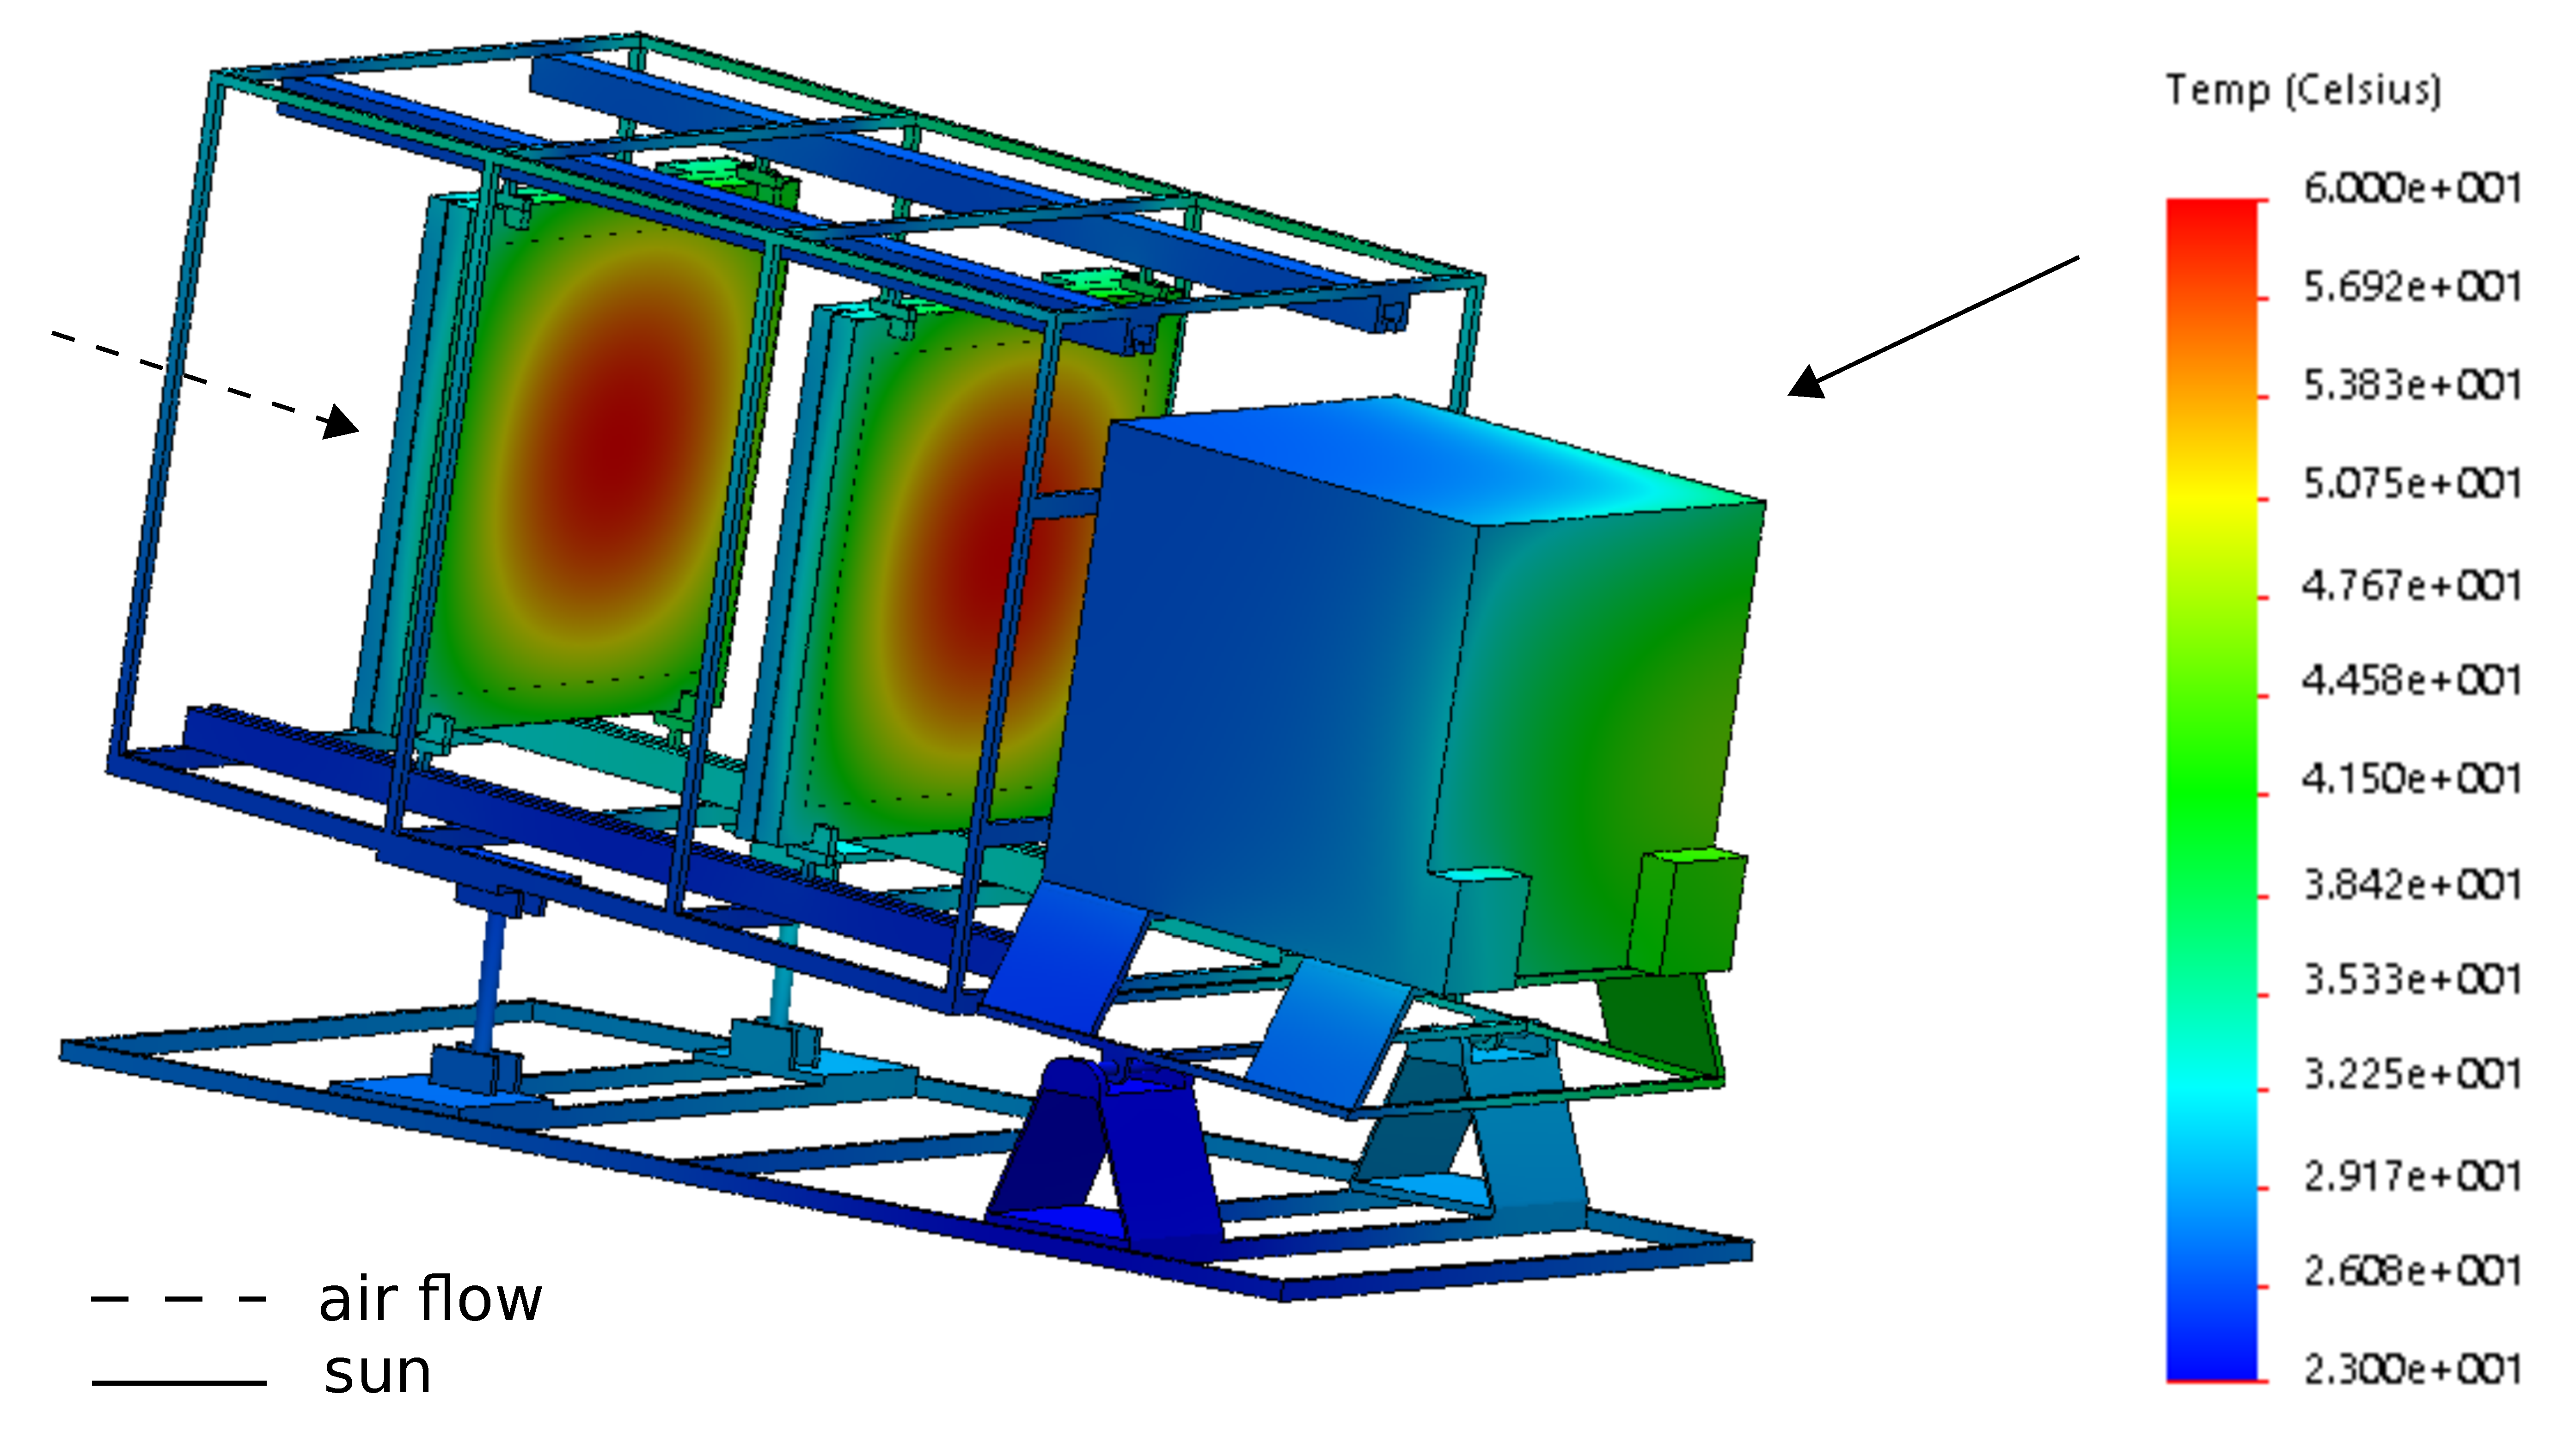
\includegraphics[width=.7\textwidth]{Figures/MuTe_Temp.eps}
\caption{Heat distribution map of the MuTe structure under typical environmental conditions at the Cerro-Machin volcano.}
\label{fig:detec} 
\end{figure}

In Figure \ref{fig:detec}, we see the temperature distribution on the MuTe structure resulting from the thermal simulation. The maximum temperature at which MuTe is subjected is around 60$^{\circ}$C in the middle of the scintillation panels because the direct incidence of the solar radiation (solid arrow). However, by means of the convection process created by the frontal wind (dashed arrow), this temperature drops to 26$^{\circ}$C. The water volume inside the WCD dissipates the heat of the stainless steel cube finding a temperature of 40 $^{\circ}$C.

\section{Temperature influence on the MuTe-SiPMs}
\label{sec:temp}

In this section, we present the analysis of temperature affectation over the most important parameters of MuTe-SiPMs such as breakdown voltage and dark count rate at the observation place.

To assess the behavior of the SiPMs under environment conditions we use temperature data recorded during the 2017 rainy season between 22-23 at the Cerro Machin volcano. The temperature had a minimum value at night of about 8.4 $^{\circ}$C and a maximum at day about 15.8 $^{\circ}$C as shown in Figure \ref{fig:temp_mach}. In the analysis, we evaluated the DCR, breakdown voltage, and gain of the MuTe SiPMs in relation with the temperature data provided by sensors (HP03) located inside the scintillation panels. 

\begin{figure}[htbp]
\centering 
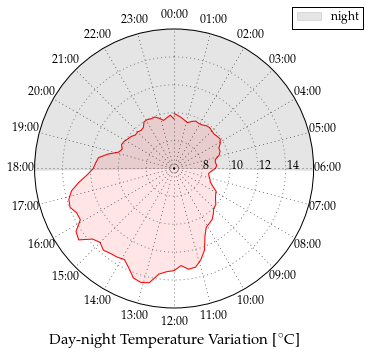
\includegraphics[width=.4\textwidth]{Figures/Temp.png}
\caption{\label{fig:temp_mach} Day-night temperature variation at the Cerro-Mach\'in volcano during the rainy season.}
\end{figure}

In Figure \ref{fig:behav} we present the nigh-day cycle variation of the breakdown voltage and DCR depending on temperature taking into account their coefficients, 41.7mV/$^{\circ}$C and 0.85kHz/$^{\circ}$C respectively.

\begin{figure}[htbp]
\centering 
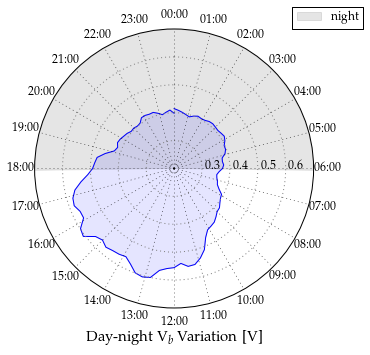
\includegraphics[width=.4\textwidth]{Figures/Vb.png}
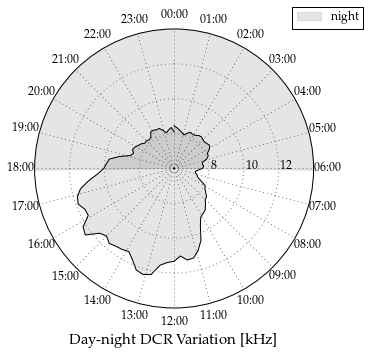
\includegraphics[width=.4\textwidth]{Figures/DCR.png}
\caption{\label{fig:behav} MuTe SiPM breakdown voltage and DCR variation as a function of typical temperature values at the Cerro-Mach\'in volcano.}
\end{figure}

We observed that the breakdown voltage changes up to $\pm$300 mV from the nominal value (53.2 V) generating a gain deviation of up to 0.77$\times 10^5$ and a DCR increasing up to 12 kHz. 

The maximum variance of the pulse amplitude is about 2 mV for a $\Delta T \sim 8 ^{\circ}$C which represents roughly 14.8$\%$ of the voltage separation between two consecutive photoelectrons ($\sim$ 13.5 mV at 56 V). If the amplitude shift exceeds the value of one photoelectron and if the discrimination threshold of the hodoscope is just above 5 p.e., the rate of the hodoscope will increase. However, in this case, the amplitude increment due to the temperature is negligible and it does not represent a risk in the hodoscope detection rate. Only, a temperature gradient higher than 50$^{\circ}$C will cause a representative rate variation.

\begin{figure}[htbp]
\centering 
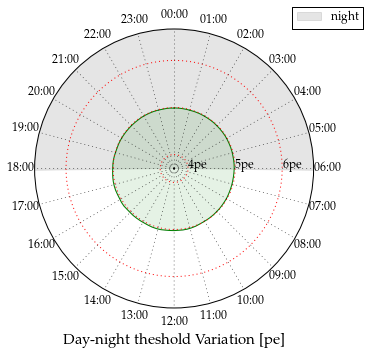
\includegraphics[width=.4\textwidth]{Figures/peT.png}
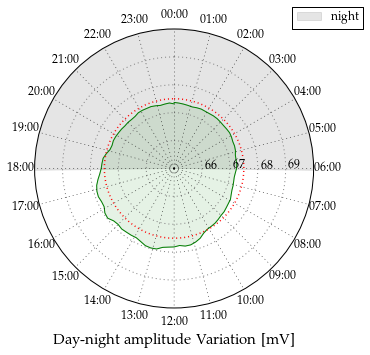
\includegraphics[width=.4\textwidth]{Figures/peakT.png}
\caption{\label{fig:thre} Photoelectron and pulse amplitude variation of the MuTe-SiPM for typical temperature values at the Cerro-Mach\'in volcano.}
\end{figure}

The MuTe hodoscope discrimination threshold was set above 5 pe = 67.5 mV in order to take out the noise contributions due to DCR, after pulse and crosstalk and their respective variations due to temperature. Figure \ref{fig:thre} shows the resulting variance around the threshold voltage (Right) and its respective photoelectron equivalent (Left). 

To assess the MuTe-SiPMs behavior in on-field conditions, we analyzed 5 days of data from 2019/12/20 to 2019/12/25. In Figure \ref{fig:temp} we show the temperature of the rear ($T_R$) and frontal ($T_F$) panels, as well as the in-coincidence detection rate of them. The MuTe was pointing towards the horizon without elevation, with an angular aperture of 52$^{\circ}$, an inter-panel separation of 2.5 m, and a discrimination threshold of 8 p.e.

\begin{figure}[htbp]
\centering 
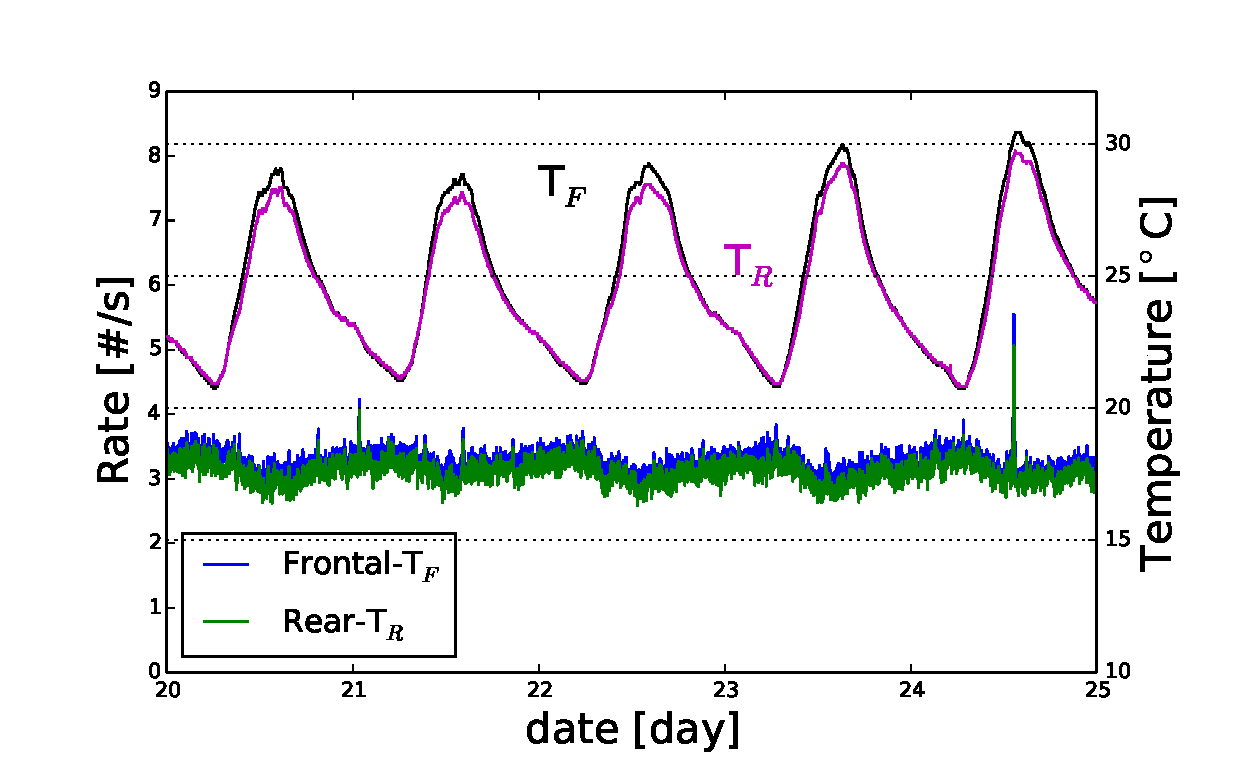
\includegraphics[width=0.7\textwidth]{Figures/Modulation.eps}
\caption{\label{fig:temp} Hodoscope rate modulation depending on the environmental temperature of the MuTe recorded from 2019/12/20 to 2019/12/25. The green line displays the rear panel rate under temperature $T_R$ and the blue line the frontal panel rate under temperature $T_F$. }
\end{figure}

The panel temperature oscillates from 20$^{\circ}$C to 30 $^{\circ}$C representing a gradient of 10$^{\circ}$C. How it was explained above, a 10$^{\circ}$C gradient represents a variation in the pulse amplitude around 14.8$\%$ which is not enough to jump between photoelectron levels. For that reason, the rate is not affected by the SiPM behavior, only by the intrinsic cosmic ray temperature modulation. When the atmospheric temperature rises up, its density decreases, reducing the particle interaction probability and the particle flux at ground level. As a consequence, the hodoscope rate experiences an inverse relation with the environmental temperature. In this case, the average flux is $\sim$3.1 events/s varying roughly 11.2$\%$ at the maximum and minimum temperature. If the SiPMs were affected by heat transfer on the structure, the hodoscope rate will increase with temperature, but that was not observed.

\section{Conclusions and Outlook}
\label{sec:conc}

We evaluated the SiPM S13360-1350CS from Hamamatsu in order to characterize the breakdown voltage, gain and noise depending on the overvoltage and temperature. Temperature testes ranged from 0$^{\circ}$C to 40$^{\circ}$C covering the temperature spectrum of the observation site at Cerro Mach\'in Volcano, Colombia. The SiPM breakdown voltage variation ratio was about 41.7mV/$^{\circ}$C indicating a pulse amplitude shift of 14.8$\%$ which is not representative for jumping between photoelectron levels. We also estimated a gain increase ratio of about 3.07$\times 10^5$/V for overvoltage changes on the SiPM. 

In the noise characterization we found that the dark count rate decreases by several magnitude orders (< 100 Hz) at a threshold above 3 p.e. On the other hand, the DCR increases with a ratio of 11.16 kHz/V as a function of the SiPM overvoltage. This proposes a trade-off challenge because temperature increase generates a breakdown voltage increase but also a rising of the DCR. In the SiPM S13360-1350CS, the afterpulse and crosstalk probabilities showed a non-linear growth with the temperature reaching up to 3$\%$ and 5$\%$ at an overvoltage of 3.7 V respectively. We recommend a discrimination threshold above 5 p.e in order to reduce drastically the correlated and non-correlated noise from MuTe SiPMs. 

In the on-field test, the hodoscope rate was modulated by the environmental temperature reaching a maximum deviation of 11.2$\%$ respect to the average. The modulation was inversely correlated to the temperature indicating that its origin is because of the cosmic ray flux variability and it is not by the SiPM behavior where the rate will be directly correlated.

%The breakdown voltage variability due to temperature needs be compensated by a closed-loop control of the SiPM bias voltage.

% \begin{table}[htbp]
% \centering
% \caption{\label{tab:summ} SiPM S13360-1350CS features at 56V/25$^{\circ}$C}
% \smallskip
% \begin{tabular}{|l|c|}
% \hline
% Parameter & Value\\
% \hline
% Breakdown voltage [V] & 52.3\\
% Gain &  1.3$\times10^6$\\
% Photo-electron equivalent [mV] &  13.5\\
% Dark Count Rate [Hz] &  2$\times10^5$\\
% Afterpulse [$\%$] &  2.9\\
% Crosstalk [$\%$] &  5\\
% \hline
% \end{tabular}
% \end{table}

%\appendix
%\section{Some title}
%Please always give a title also for appendices.

\acknowledgments

The authors acknowledge the financial support of  Departamento Administrativo de Ciencia, Tecnolog\'ia e Innovaci\'on of Colombia (ColCiencias) under contract FP44842-082-2015 and to the Programa de Cooperaci\'on Nivel II (PCB-II) MINCYT-CONICET-COLCIENCIAS 2015, under project CO/15/02.





% We suggest to always provide author, title and journal data:
% in short all the informations that clearly identify a document.

\bibliographystyle{unsrt}
\bibliography{MuTe.bib}

\end{document}

